\documentclass[12pt]{beamer}
\usepackage{subcaption}
\usepackage[magyar]{babel}
\usepackage{t1enc}
\usepackage{tikz}
\usepackage{xcolor}
\usepackage{pgfplots}
\pgfplotsset{compat=1.18}
\usetheme{Berkeley}
\usecolortheme{default}
\definecolor{maroon}{rgb}{0.5, 0.0, 0.0}
\definecolor{mathgreen}{HTML}{509600}
%\setbeamercovered Nincs rá szükségünk
%\newtheorem{tetel}{Tétel}

\begin{document}
	\author{Szabó András \& Sándor Máté}
	\title{tikz \& pgfplots}
	%\subtitle{Bevezetés a \TeX-be} Nincs rá szükségünk
	\date{2021/22/I.\ félév}
	\institute{Miskolci Egyetem Sztárképző}
	\frame[plain]{\maketitle}
	
	%tableofcontent nem kell nekünk
	
	%Egyenletek létrehozása a Tikz és Pgfplots segítségével
	\section{Szakasz}
	\subsection{Alszakasz}
	\begin{frame}{PROBA FRAME}
		\begin{columns}[T] % align columns
			\begin{column}{.48\textwidth}
				\color{gray}
				
				{\huge PDF Nézet}
				
				\rule{\linewidth}{3pt}
				
				TODO-LEFT
				
				
			\end{column}%
			\hfill%
			\begin{column}{.48\textwidth}
				\color{blue}
				
				{\huge \TeX \! Kód}
				
				
				\rule{\linewidth}{3pt}
				
				TODO-RIGHT
				
				
			\end{column}%
		\end{columns}
	\end{frame}
	
	\section{Paragrafusok}
	\subsection{Paragrafus txt-ből}
	\begin{frame}{Paragrafus txt-ből}
		\begin{columns}[T] % align columns
			\begin{column}{.48\textwidth}
				{\color{gray}
				
				{\huge PDF Nézet}
				
				\rule{\linewidth}{3pt}}
				
				\begin{tikzpicture}[scale=0.50]
					\begin{axis}[
						title={\LARGE TXT Paragrafus},
						xlabel={$x$},
						ylabel={$y$},
						]
						\addplot[blue]table {adat.txt};
					\end{axis}
				\end{tikzpicture}
				
				
			\end{column}%
			\hfill%
			\begin{column}{.48\textwidth}
				{\color{blue}
				
				{\huge \TeX \! Kód}
				
				\rule{\linewidth}{3pt}}
				
				{\color{cyan}\textbackslash begin\{{\color{blue}tikzpicture}\}
				
					{\color{maroon}\quad {\color{orange} \textbackslash begin}\{axis\}[
					
						title=TXT Paragrafus,
						
						xlabel={{\color{mathgreen}\$x\$}},
						
						ylabel={{\color{mathgreen}\$y\$}},]
						
						{\color{orange}\textbackslash addplot}[blue]table \{adat.txt\};
						
					{\color{orange}\quad\textbackslash end}\{axis\}
					
				\textbackslash end\{{\color{blue}tikzpicture}\}}}
				
				
			\end{column}%
		\end{columns}
	\end{frame}

	\subsection{Négyzetfüggvény}
		\begin{frame}{Négyzetfüggvény}
		\begin{columns}[T] % align columns
			\begin{column}{.48\textwidth}
				\color{gray}
				
				{\huge PDF Nézet}
				
				\rule{\linewidth}{3pt}
				
				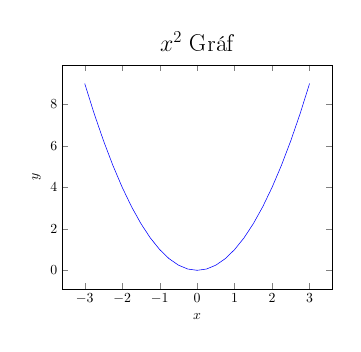
\begin{tikzpicture}[scale=0.50]
					\begin{axis}[
						title={\LARGE $x^2$ Gráf},
						xlabel={$x$},
						ylabel={$y$},
						]
						\addplot[blue,domain=-3:3] {x^2};
					\end{axis}
				\end{tikzpicture}
				
				
			\end{column}%
			\hfill%
			\begin{column}{.48\textwidth}
				{\color{blue}
					
					{\huge \TeX \! Kód}
					
					\rule{\linewidth}{3pt}}
				
				{\color{cyan}\textbackslash begin\{{\color{blue}tikzpicture}\}
					
					{\color{maroon}\quad {\color{orange} \textbackslash begin}\{axis\}[
						
						title={{\color{mathgreen}\$x \^\ 2\$}},
						
						xlabel={{\color{mathgreen}\$x\$}},
						
						ylabel={{\color{mathgreen}\$y\$}},]
						
						{\color{orange}\textbackslash addplot}[blue,domain=-3:3] \{x \^\ 2\};
						
						{\color{orange}\quad\textbackslash end}\{axis\}
						
						\textbackslash end\{{\color{blue}tikzpicture}\}}}
				
				
			\end{column}%
		\end{columns}
	\end{frame}

	\subsection{Több függvény egy ábrán}
	\begin{frame}{Több függvény egy ábrán}
		\begin{columns}[T] % align columns
			\begin{column}{.48\textwidth}
				\color{gray}
				
				{\huge PDF Nézet}
				
				\rule{\linewidth}{3pt}
				
				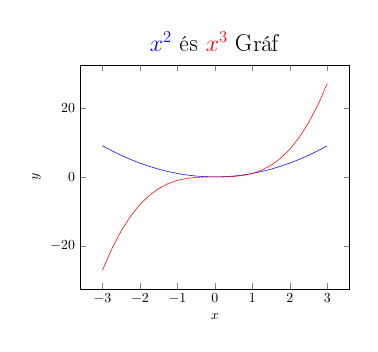
\begin{tikzpicture}[scale=0.50]
					\begin{axis}[
						title={\LARGE {\color{blue}$x^2$} és {\color{red}$x^3$} Gráf},
						xlabel={$x$},
						ylabel={$y$},
						]
						\addplot[blue,domain=-3:3] {x^2};
						\addplot[red,domain=-3:3] {x^3};
					\end{axis}
				\end{tikzpicture}
				
				
			\end{column}%
			\hfill%
			\begin{column}{.48\textwidth}
				{\color{blue}
				
				{\huge \TeX \! Kód}
				
				\rule{\linewidth}{3pt}}
			
		{\color{cyan}\textbackslash begin\{{\color{blue}tikzpicture}\}
		
		{\color{maroon}\quad {\color{orange} \textbackslash begin}\{axis\}[
			
			title={{\color{mathgreen}\$x \^\ 2\$}},
			
			xlabel={{\color{mathgreen}\$x\$}},
			
			ylabel={{\color{mathgreen}\$y\$}},]
			
			{\color{orange}\textbackslash addplot}[blue,domain=-3:3] \{x \^\ 2\};
			{\color{orange}\textbackslash addplot}[red,domain=-3:3] \{x \^\ 3\};
			
			{\color{orange}\quad\textbackslash end}\{axis\}
			
			\textbackslash end\{{\color{blue}tikzpicture}\}}}
				
				
			\end{column}%
		\end{columns}
	\end{frame}

	
	
	
	
	
\end{document}